\section{The System}

% High-level architecture

\begin{figure}
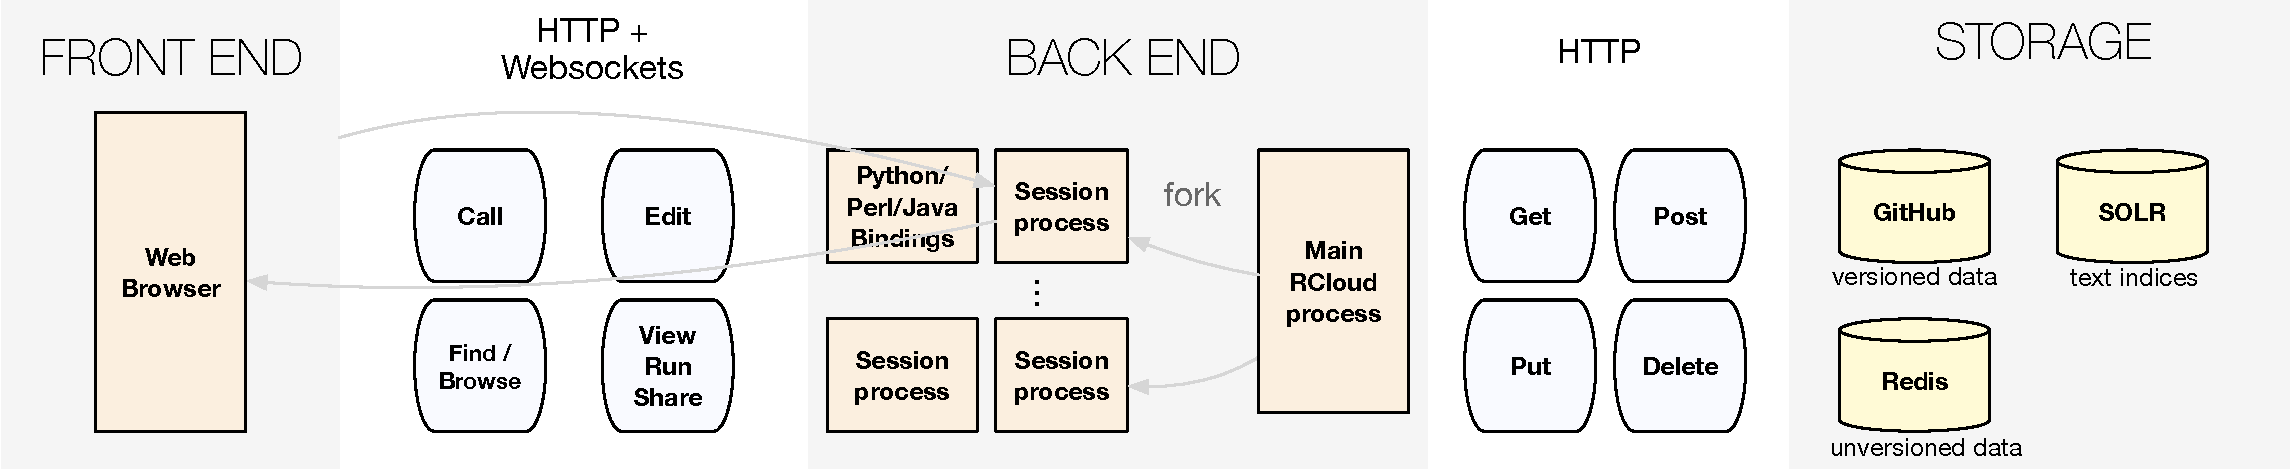
\includegraphics[width=\linewidth]{fig/system/system.pdf}
\caption{\label{fig:system}A diagram of RCloud's architecture. Dashed
  lines represent features which not yet implemented.}
\end{figure}

The internal computing infrastructure of organizations has changed
radically in the last fifteen years. The shift from large
servers toward scalable, lower-cost, distributed systems (``the cloud'')
led to a software ecosystem of processes distributed over a
network (often virtually defined) communicating via some
high-level protocol, usually HTTP.  HTTP is dominant because web
browsers and servers are ubiquituous and available in essentially
all hardware devices, from tiny sensors, to handheld devices and
laptops, to rack-mounted servers.

As a result, HTTP is the lingua franca of interprocess communication
(IPC). One of the design goals for RCloud was to provide an attractive
environment for creators of data-analysis scripts, that also behaves
as a first-class citizen in the pre-existing ecosystem of computer
services and networks with an organization.

%% Design for cloud-friendly? This goes back to the point in the
%% introduction about playing nice with the rest of the ecosystem.

\subsection{System Design}

We designed RCloud around the front-facing API, which provides roughly
one entry point to correspond with each requirement.

Edit

View/Run/Share

Call

Browse/Search. ``More like this'', and a custom webpage solely for browsing.

\subsection{Notebooks\label{sec:notebooks}}

Notebooks as Github gists. 
%
We needed version control over a directory, gist provides that,
wrapped over an HTTP interface.
%
Mainly a tactical decision to save time.
%
Nevertheless, availability of notebook data as (barely) plain text had good side
effects, like ease to build search. 
%
Expect same with suggest.

\subsection{Reputation and Interest: starring\label{sec:starring}}

In RCloud, reputation and interest are a relationship between
\emph{notebooks} and \emph{users}, rather than a relationship between
user pairs. We decided on this approach because we expect typical
RCloud deployments to have relatively few users, but each user to have
written relatively many notebooks. Under that assumption, assigning
interest to users would not provide sufficiently ``high-resolution'' data.

We incorporate both explicit and implicit indications of interest
in notebooks. Explicit interest is signalled by ``starring,'' or
clicking on a button that marks a notebook as interesting. 
This makes explicit indication of interest a nearly trivial operation,
always readily available, thus encouraging its use.

Implicit signaling of interest is supported by keeping click-through
\cite{Joachims:2005:AIC} and execution counts. (In addition to these
classic web search techniques of collecting feedback, we have the
prospect of applying static and dynamic code analysis to generate
further fine-grained information about relationships, for example,
which packages and data sets often appear together.)

\todo{explain} These will be ingredients for the recommendation system.

\subsection{Deployment of notebooks\label{sec:deployment}}

Notebooks as versioned subroutines, web services.

There exists a URL for every notebook in RCloud, and notebooks by
default are visible by the entire organization. This is deliberate.
As pointed out by Wattenberg and Kriss~\cite{Wattenberg:2011:DFS},
broad access to analysis outputs (in their case, for NameVoyager)
increases long-term engagement in part through crossreferences on
the web. Although our prototype RCloud deployment is only visible
inside a corporate intranet, we nevertheless found anecdotal support
for this notion by discovering links to RCloud notebooks in internal
discussion fora and mailing lists.

\subsection{Technologies: R, Python, HTML5, interactive notebooks, etc.}

How do we do things that are not trivial to do with IPython (for example)

dcplot. two-way communication between between backend session and
frontend session.

A key engineering decision in RCloud was to rely on full two-way
communication between human interface in a web client, and remote
data and computing resources in the cloud.
